\documentclass[tikz,border=9pt]{standalone}
\usepackage[utf8]{inputenc}
\usepackage[OT4,plmath]{polski}
\usepackage{amsmath}
\begin{document}
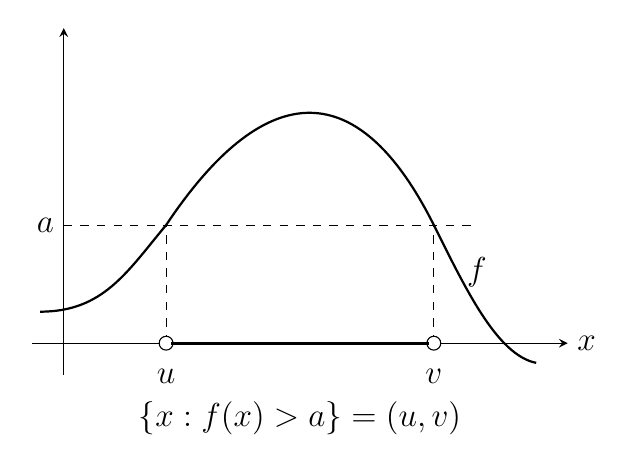
\begin{tikzpicture}[font=\large,>=stealth]
  \draw[->] (-0.4,0)--(6.4,0) node[right] {$x$};
  \draw[->] (0,-0.4)--(0,4.0);
  \draw[dashed] (0,1.5)--(5.2,1.5);
  \node[left] at (0,1.5) {$a$};
  \draw[thick] (-0.3,0.4)..controls (0.5,0.4) and (0.8,0.9)..(1.3,1.5)
    ..controls (2.5,3.3) and (3.7,3.5)..(4.7,1.5)
    ..controls (5.1,0.7) and (5.5,-0.15)..(6,-0.25);
  \node[right] at (5.0,0.9) {$f$};
  \foreach \x in {1.3,4.7} {
    \draw[dashed] (\x,0)--(\x,1.5);
    \node[circle,draw,fill=white,inner sep=0pt,minimum size=5pt] at (\x,0) {};
  }
  \draw[very thick] (1.36,0)--(4.64,0);
  \node[below=6pt] at (1.3,0) {$u$};
  \node[below=6pt] at (4.7,0) {$v$};
  \node at (3,-0.95) {$\{x:f(x)>a\}=(u,v)$};
\end{tikzpicture}
\end{document}
